\documentclass[a4paper]{article}
\usepackage{listings}
\usepackage{qtree}
\usepackage{xcolor}
\usepackage{forest}
\usepackage{multicol}
\setlength{\columnsep}{3cm}
\usepackage{parskip}
\usepackage{changepage}
\usepackage[T1]{fontenc}
\usepackage{amsmath}
\usepackage{hyperref}
\usepackage{listings}
\usepackage{amsthm}
\usepackage{amssymb}
\usepackage{float}
\usepackage[utf8]{inputenc}
\usepackage{graphicx}
\usepackage[italian]{babel}
\usepackage{thmtools}
\graphicspath{{figures/}}
\newcommand{\channel}{\textit{channel }}
\newcommand{\pacchetto}{\textit{pacchetto }}

\begin{document}

\author{Lorenzo Dentis, lorenzo.dentis@edu.unito.it}
\title{Esercizi con Uppaal}
\maketitle
%http://ppedreiras.av.it.pt/resources/empse0809/slides/TheUppaalModelChecker-Julian.pdf
\section{Modello A}
Stop and wait e canale perfetto.\\ 
Si assume che il canale sia perfetto, e quindi nè il messaggio, nè l’ack possono essere persi. 
Il tempo di trasmissione sul link è variabile all’interno di un intervallo limitato (costanti minTransmissionTime e maxTransmissionTime ), con una differenza $\leq \frac{1}{10}$ tempo di trasmissione. 

Si definiscano e provino le proprietà di corretto funzionamento del protocollo, ini particolare si provi qual è il tempo minimo e massimo che intercorre dalla spedizione di un messaggio alla ricezione del suo ack.
\subsection{Mittente}
\begin{center}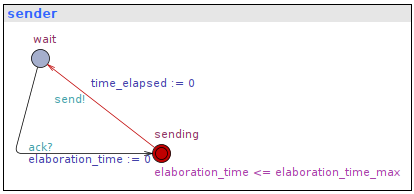
\includegraphics[width=0.8\textwidth]{1_sender.png}\end{center}
Il Mittente prepara un messaggio,lo invia e rimane in attesa di ricevere un Acknowledgment, per poterlo inviare si sincronizza sul \channel send (tramite \texttt{send!}) e per ricevere l'ack si sincronizza sul \channel ack (tramite \texttt{ack?}).\\
Quando un messaggio viene invato viene avviato un timer, \textit{time\_elapsed}, che sarà utile in fase di analisi per stabilire quanto tempo è passato dall'invio del messaggio alla ricezione dell'ack.
Il Mittente può rimanere in stato di elaborazione un tempo inferiore ad una costante \textit{elaboration\_time\_max}, quindi vi è un altro clock \textit{elaboration\_time} che viene resettato ogni volta che viene ricevuto un ack.
In tal modo il Mittente non può rimanere all'infinito in fase di elaborazione.
\subsection{Destinatario}
\begin{center}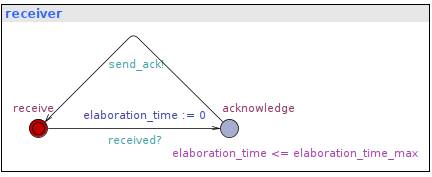
\includegraphics[width=0.8\textwidth]{1_receiver.png}\end{center}
Il Destinatario può solo attendere la sincronizzazione sul \channel received, quando il canale gli fornisce un messaggio il Destinatario risponde con un Acknowledgment che viene inviato sul canale sincronizzandosi sul \channel send\_ack.\\
Il Destinatario può rimanere in stato di elaborazione un tempo inferiore ad una costante \textit{elaboration\_time\_max}, quindi vi è un altro clock \textit{elaboration\_time} che viene resettato ogni volta che viene ricevuto un messaggio.
In tal modo il Destinatario non può rimanere all'infinito in fase di elaborazione.
\subsection{Canale}
Il canale presentato è un canale perfetto, quindi riceve un messaggio o un ack e lo consegna senza possibilità di perderlo.
Il canale è half-duplex, quindi permette la trasmissione non simultanea sia da Mittente a Destinatario che viceversa.\\
\begin{center}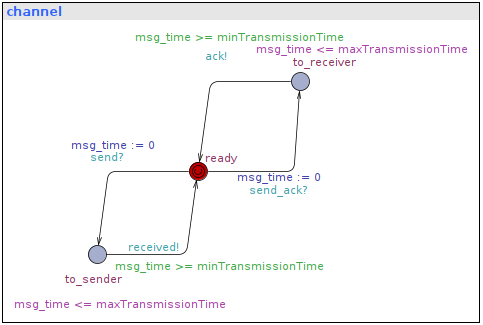
\includegraphics[width=1\textwidth]{channel_safe.png}\end{center}
Il canale quando non sta trasmettendo un messaggio si trova nello stato \textit{ready}, se il messaggio proviene dal Mittente il canale si sincronizza sul \channel send e si sposta nello stato \texttt{to\_sender}, da questo stato esce solo dopo \textit{minTransmissionTime} e prima di \textit{maxTransmissionTime}, per rappresentare il tempo di trasmissione varibile del canale.
Per consegnare il messaggio si sincronizza con il Destinatario sul \channel received.\\
Discorso diametralmente opposto vare per l'Acknowledgment, il canale si sincroniza con il Destinatario sul \channel send\_ack, e consegna l'ack dopo un intervallo di tempo sincronizzandosi con il Mittente sul \channel ack.
In ultimo è presente un timer che viene resettato sull'arco di "presa in carico" di un \pacchetto, questo timer può esssere utilizzato per verificare il tempo necessario alla trasmissione di un singolo \pacchetto.
\subsection{Analisi}
\begin{itemize}
	\item \textit{A[] not deadlock}\\
		Il sistema non presenta stati di deadlock.
	\item \textit{sender.sending --> ((time\_elapsed >= 2 * minTransmissionTime \&\& time\_elapsed <= 2 * (maxTransmissionTime + elaboration\_time\_max)) ||(time\_elapsed <= elaboration\_time\_max))}\\
		Quando il Mittente si trova nello stato \textit{sending} il tempo trascorso può avere solo due valori: [0,elaboration\_time\_max] se non è ancora stato inviato nessun messaggio, oppure un valore compreso tra 2* tempo di trasmissione minimo e 2* tempo di trasmissione massimo + il tempo di elaborazione. Infatti, perchè il Mittente consideri il messaggio ricevuto e torni nello stato prepare, deve aver ricevuto un ack, il tempo per ricevere un ack è il doppio del tempo necessario a trasmettere un \pacchetto (considerando anche l'elaborazione)
	\item \textit{sender.sending --> sender.sending \&\& time\_elapsed > elaboration\_time\_max}\\
		Questa condizione è verificata in quanto se invio un messaggio (quindi il tempo di elaborazione è stato superato) ottengo un ack. 
	\item \textit{sender.sending --> receiver.acknowledge}\\
		Questa condizione è verificata in quanto se invio un messaggio il Destinatario lo riceve.
	\item \textit{channel.to\_sender --> channel.to\_receiver}\\
		Questa verifica è effettuata per assicurarsi che in questo sistema quando il canale prende in carico un messaggio lo consegna sempre al Destinatario.
	\item \textit{channel.ready --> (channel.ready \&\& msg\_time >= minTransmissionTime \&\& msg\_time <= maxTransmissionTime + elaboration\_time\_max)}\\
		Questa condizione è verificata perchè se parto da uno stato in cui il canale e pronto a trasmettere tornerò dopo qualsiasi esecuzione ad essere pronto a trasmettere dopo un tempo compreso tra maxTrasmissione (considerando l'elaborazione) e minTrasmissione.
		Qualsiasi sia l'agente che ha inviato in \pacchetto.
\end{itemize}

\section{Modello B}
Stop and wait e canale rumoroso.\\ 
In questo modello sia il messaggio che il realtivo Acknowledgment possono essere smarriti, ma il protocollo non è stato modificato in alcun modo per far fronte a questa situazione
Il tempo di trasmissione sul link è variabile all’interno di un intervallo limitato (costanti minTransmissionTime e maxTransmissionTime ), con una differenza $\leq \frac{1}{10}$ tempo di trasmissione. 

Si definiscano e provino le proprietà di corretto funzionamento del protocollo, in particolare si provi qual è il tempo minimo e massimo che intercorre dalla spedizione di un messaggio alla ricezione del suo ack.
\subsection{Mittente}
\begin{center}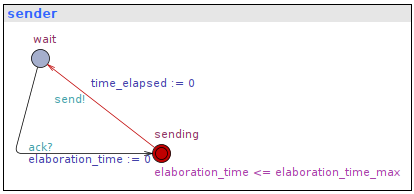
\includegraphics[width=0.8\textwidth]{1_sender.png}\end{center}
Il Mittente prepara un messaggio,lo invia e rimane in attesa di ricevere un Acknowledgment, per poterlo inviare si sincronizza sul \channel send (tramite \texttt{send!}) e per ricevere l'ack si sincronizza sul \channel ack (tramite \texttt{ack?}).
Quando un messaggio viene invato viene avviato un timer, \textit{time\_elapsed}, che sarà utile in fase di analisi per stabilire quanto tempo è passato dall'invio del messaggio alla ricezione dell'ack.
Il Mittente può rimanere in stato di elaborazione un tempo inferiore ad una costante \textit{elaboration\_time\_max}, quindi vi è un altro clock \textit{elaboration\_time} che viene resettato ogni volta che viene ricevuto un ack.
In tal modo il Mittente non può rimanere all'infinito in fase di elaborazione.
\subsection{Destinatario}
\begin{center}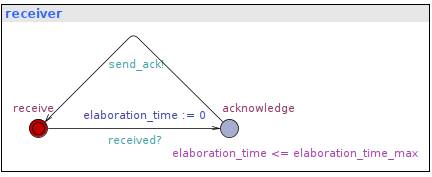
\includegraphics[width=0.8\textwidth]{1_receiver.png}\end{center}
Il destinatario può solo attendere la sincronizzazione sul \channel received, quando il canale gli fornisce un messaggio il Destinatario risponde con un Acknowledgment che viene inviato sul canale sincronizzandosi sul \channel send\_ack.
Il Destinatario può rimanere in stato di elaborazione un tempo inferiore ad una costante \textit{elaboration\_time\_max}, quindi vi è un altro clock \textit{elaboration\_time} che viene resettato ogni volta che viene ricevuto un messaggio.
In tal modo il Destinatario non può rimanere all'infinito in fase di elaborazione.
\subsection{Canale}
Il canale è half-duplex, quindi permette la trasmissione non simultanea sia da Mittente a destinatario che viceversa.
Il canale è "rumoroso", cioè un \textit{\pacchetto}può venir perso, sia questi un messaggio o un ack. Quindi il canale può passare dallo stato che rappresenta la presa in carico allo stato ready senza effettivamente consegnare il \pacchetto.\\
\begin{center}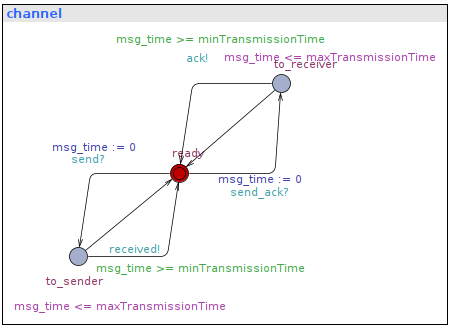
\includegraphics[width=1\textwidth]{channel_unsafe.png}\end{center}
Il canale quando non sta trasmettendo un messaggio si trova nello stato \textit{ready}, se il messaggio proviene dal Mittente il canale si sincronizza sul \channel send e si sposta nello stato \texttt{to\_sender}, da questo stato esce solo dopo \textit{minTransmissionTime} e prima di \textit{maxTransmissionTime}, per rappresentare il tempo di trasmissione varibile del canale.
Per consegnare il messaggio si sincronizza con il Destinatario sul \channel received.\\
discorso diametralmente opposto vare per l'Acknowledgment, il canale si sincroniza con il Destinatario sul \channel send\_ack, e consegna l'ack dopo un intervallo di tempo sincronizzandosi con il Mittente sul \channel ack.
É poi presente un timer che viene resettato sull'arco di "presa in carico" di un \pacchetto, questo timer può esssere utilizzato per verificare il tempo necessario alla trasmissione di un singolo \pacchetto.
In ultimo sono presenti due archi che vanno dagli stati di presa in carico (\textit{to\_sender} e \textit{to\_receiver}) allo stato \textit{ready} senza sincronizzarsi con il Mittente o con il Destinatario, quindi di fatto senza consegnare il \pacchetto.

\subsection{Analisi}
\begin{itemize}
	\item \textit{A[] not deadlock}\\
		Il sistema presenta diversi stati di deadlock. Tutte le tracce in cui un \pacchetto viene smarrito, la traccia che porta più rapidamente al deadlock è la seguente:
		$$ sender.sending \rightarrow channel.to\_send \rightarrow channel.ready $$
		In questa situazione il sistema non può più evolvere dato che il Mittente attende il canale per sincronizzarsi su \channel ack ma il Mittente non ci arriverà mai dato che è bloccato dal Mittente che sta aspettando la sincronizzazione sul \channel received.
	\item \textit{A[] sender.prepare imply ((time\_elapsed >= 2 * minTransmissionTime \&\& time\_elapsed <= 2 * maxTransmissionTime) || time\_elapsed == 0)}\\
		Nonostante ci siano dei deadlock questa proposizione è sempre verificata, infatti se un messaggio è stato consegnato ed il relativo ack è giunto al Mittente abbiamo la sicurezza che i limiti di trasmissione sono stati rispettati, in quanto non si è verificato deadlock.
		Se si fosse verificato un deadlock il Mittente non avrebbe ricevuto Acknowledgement.
	\item \textit{sender.sending --> sender.sending \&\& time\_elapsed > elaboration\_time\_max}\\
		Questa condizione non è verificata in quanto potrei perdere il messaggio o l'ack.
	\item \textit{sender.sending --> receiver.acknowledge}\\
		Questa condizione non è verificata in quanto se invio un messaggio non è detto che il Destinatario lo riceva.
	\item \textit{channel.to\_sender --> channel.to\_receiver}\\
		Questa condizione non è verificata in quanto in questo sistema quando il canale prende in carico un messaggio non c'è garanzia che lo consegni al Destinatario
	\item \textit{channel.ready --> (channel.ready \&\& msg\_time >= minTransmissionTime \&\& msg\_time <= maxTransmissionTime + elaboration\_time\_max)}\\
		Questa condizione non è verificata poichè in caso di deadlock il timer \textit{msg\_time} supera il limite massimo di trasmissione.
		Attenzione, non è vera la neagazione di questa proposizione, tutte le tracce che non vanno in deadlock rendono vera la proposizione.
\end{itemize}


\section{Modello c}
Stop and wait con ritrasmissione e canale rumoroso.\\
In questo modello sia il messaggio che il realtivo Acknowledgment possono essere smarriti, ma il protocollo è stato modificato in modo da ritrasmettere il messaggio in caso un ack non venga ricevuto entro un dato tempo limite, evento chiamato \textit{timeout}.
Il tempo di trasmissione sul link è variabile all’interno di un intervallo limitato (costanti minTransmissionTime e maxTransmissionTime ), con una differenza $\leq \frac{1}{10}$ tempo di trasmissione.

Si definiscano e provino le proprietà di corretto funzionamento del protocollo, in particolare si provi qual è il tempo minimo e massimo che intercorre dalla spedizione di un messaggio alla ricezione del suo ack e ci si assicuri che viene ricevuto l'ack corrispondente al frame inviato.
\subsection{Mittente}
Il Mittente è molto differente in questo modello, in quanto deve implementare il meccanismo di timeout.
\begin{center}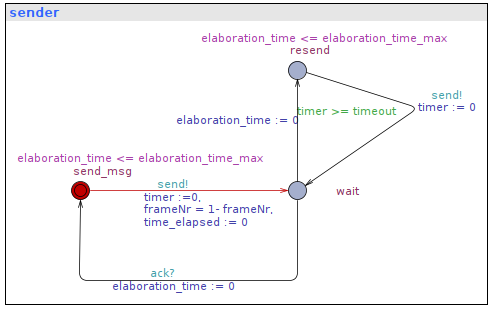
\includegraphics[width=0.8\textwidth]{2_sender.png}\end{center}
Il Mittente prepara un messaggio e lo invia sincronizzandosi sul \channel send (tramite \texttt{send!}).
Quando un messaggio viene invato viene avviato un timer, \textit{time\_elapsed}, che sarà utile in fase di analisi per stabilire quanto tempo è passato dall'invio del messaggio alla ricezione dell'ack, il \texttt{frameNr} viene modificato per identificare il nuovo messaggio e viene avviato un timer che servirà per implementare il meccanismo di timeout.
Una volta spedito il messaggio si mette in attesa dell'ack nello stato \textit{wait} da cui può uscire in due modi: grazie alla ricezione di un ack dal canale (cioè la sincronizzazione sul \channel ack) oppure per il superamento del valore di timeout.\\
Se il timeout viene superato il Mittente si sposta su uno stato \textit{resend} e ripete l'invio del messaggio resettando il timer e sincronizzandosi con il canale sul \channel send.
Il timeout causa diversi comportamenti a seconda del valore a cui è impostato.
\begin{itemize}
	\item $timeout < 2 * minTransmissionTime$ In questo caso il timeout avviene in ogni caso, non permettendo l'invio di alcun messaggio.
	\item $timeout \in [minTransmissionTime, 2 * (maxTransmissionTime + elaboration\_time\_max)]$ In questo caso un timeout può verificarsi sia perchè il messaggio è stato smarrito ma anche perchè il messaggio è stato recapitato con troppo ritardo.
	\item $timeout > 2 * (maxTransmissionTime + elaboration\_time\_max)$ In questo caso non si verifica mai un timeout a meno che il messaggio non venga perso.
\end{itemize}
Il Mittente può rimanere in stato di elaborazione un tempo inferiore ad una costante \textit{elaboration\_time\_max}, quindi vi è un altro clock \textit{elaboration\_time} che viene resettato ogni volta che viene ricevuto un ack o viene effettuata una ritrasmissione.
In tal modo il Mittente non può rimanere all'infinito in fase di elaborazione.
\subsection{Destinatario}
Il Destinatario è invece molto simile a quello dei casi precedenti.
\begin{center}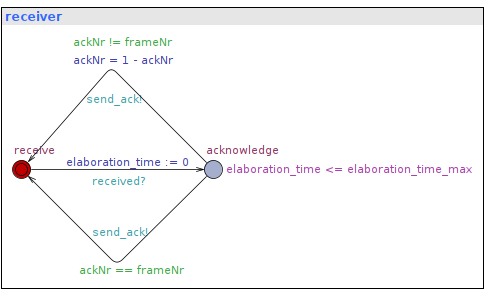
\includegraphics[width=0.8\textwidth]{2_receiver.png}\end{center}
Il destinatario può solo attendere la sincronizzazione sul \channel received, quando il canale gli fornisce un messaggio il Destinatario risponde con uno tra due tipi di Acknowledgment inviato sul canale sincronizzandosi sul \channel send\_ack.\\
I due tipi di Acknowledgment differiscono nel loro \texttt{ackNr}, una variabile che identifica il numero identificativo dell'ack.
Se l'ack fa riferimento ad un messaggio non ancora ricevuto viene eseguito l'arco "superiore" e l' \texttt{ackNr} viene modificato, in caso di messaggio già ricevuto viene invece invato un ack avente numero identificativo identico al precedente (\texttt{ackNr} non viene modificato).\\
Il Destinatario può rimanere in stato di elaborazione un tempo inferiore ad una costante \textit{elaboration\_time\_max}, quindi vi è un altro clock \textit{elaboration\_time} che viene resettato ogni volta che viene ricevuto un messaggio.
In tal modo il Destinatario non può rimanere all'infinito in fase di elaborazione.

\subsection{Analisi}
\begin{itemize}
	\item \textit{A[] not deadlock}\\
		Il sistema non va mai in deadlock
	\item \textit{sender.wait --> sender.send\_msg}\\
		Se il Mittente inva un messaggio riceve un ack. questa proposizione non è verificata in quanto esiste una esecuzione in cui nessun messaggio viene recapitato e qualunque re-invio risulta futile perchè si perde.
	\item \textit{sender.wait --> receiver.acknowledge}\
		Se il Mittente invia un messaggio il Destinatario lo riceve. Anche questa proposizione non è vera, sempre per la presenza di esecuzioni in cui tutti i messaggi vengono persi
	\item \textit{A[] sender.send\_msg imply ((time\_elapsed >= 2 * minTransmissionTime \&\& time\_elapsed <= 2 * (maxTransmissionTime + elaboration\_time\_max)) || time\_elapsed <= elaboration\_time\_max)}\\
		Di conseguenza anche questa affermazione risulta falsa, infatti non è vero che se il Mittente invia un messaggio otterrà una risposta in un dato intervallo di tempo, poichè potrebbe proprio non ricevere alcun ack.
	\item \textit{E<> (sender.wait \&\& (time\_elapsed >= 2* minTransmissionTime \&\& time\_elapsed <= 2* (maxTransmissionTime + elaboration\_time\_max)))}\\
		È invece verificata questa proposizione, in quanto esiste una esecuzione in cui il Mittente invia un messaggio e lo riceve entro l'intervallo prestabilito.
	\item \textit{sender.send\_msg --> (sender.timer >= 2* minTransmissionTime \&\& sender.timer <= 2* (maxTransmissionTime + elaboration\_time\_max) || time\_elapsed <= elaboration\_time\_max ) }\\
		Quest'ultima proposizione riguardante lo studio del tempo di trasmissione va ad identificare quali sono le esecuzioni che garantiscono la ricezione entro l'intervallo di tempo predefinito, ed è verificata.
		Queste esecuzioni sono tutte le esecuzioni in cui si riceve un ack, se si riceve un ack sicuramente lo si riceve entro un intervallo [ 2 *minTrasnsmissionTime, 2* ( maxTransmissionTime + elaborationi\_time\_max)].\\
		L'affermazione "è stato ricevuto un ack" è codificata in logica dalla proposizione \textit{"sender.send\_msg -->"} unita all'operatore logico or alla fine della proposizione.
		Infatti se il Mittente si trova nella posizione \textit{sender.send\_msg} o è perchè nessun messaggio è ancora stato spedito ( e quindi time\_elapsed $\leq$ elaboration\_time\_max ) oppure perchè è stato spedito un messaggio ed è stato ricevuto un ack.
	\item \textit{A[] sender.send\_msg imply (frameNr == ackNr)}\\
		Ogni ack ricevuto deve corrispondere al messaggio inviato, quindi il \textit{frame number} e l' \textit{acknowledgment number} devono essere uguali quando l'ack viene conseganto al Mittente.
		Come analizzato nella query precendete si può indicare la conclusione di una "trasmissione" (o il fatto che non vi è ancora stata nessuna trasmissione) scrivendo \textit{sender.send\_msg implica p} dove $p$ è una proposizione.

\end{itemize}
\end{document}
